\documentclass[../main.tex]{subfiles}

\graphicspath{{\subfix{../images/}}}

\begin{document}

\section{Task 3.4}

Create a cycle accurate communication model of a master and slave module that uses the Avalon Streaming Bus Interface (ST). Simulate that a master are transmitting data to a slave module as illustrated in Figure (\ref{fig:avalon}). The slave should store received data from the master in a text file. Include in the model a situation where the data sink signals $\text{ready} = \text{'0'}$. The simulated result should be presented in the GTK wave viewer, so a VCD trace file must be created. It should e possible to configure the channel, error and data size define in a separate header file.

\begin{figure}[h]
    \centering
    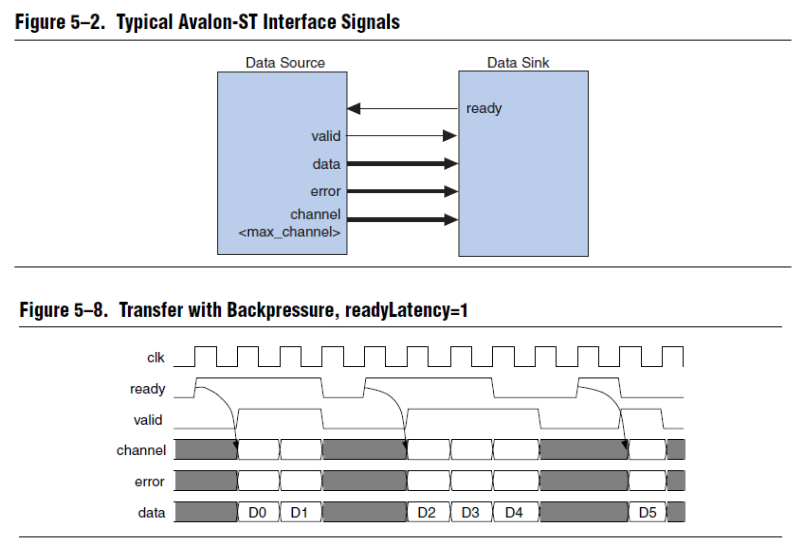
\includegraphics[width=0.85\textwidth]{task3_4.png}
    \caption{Avalon Streaming Bus Interface.}
    \label{fig:avalon}
\end{figure}

\subsection*{Solution}

We started by creating a \texttt{AvalonConf.hpp} header for containing channel defines. It also creates a typedef depending on the width of the data channel. The interface supports a data width of 8, 16, 32 and 64 bits.

\begin{myminted}{/inc/AvalonConf.hpp}
/* Avalon Channel Configuration */
#define CHANNEL_BITS    4   /* Number of channel wires      */
#define ERROR_BITS      2   /* Number of error wires        */
#define DATA_BITS       16  /* Number of data wires         */
#define MAX_CHANNEL     2   /* Maxinum number of channels   */

#if DATA_BITS == 8
typedef uint8_t binMessageType;
#elif DATA_BITS == 16
typedef uint16_t binMessageType;
#elif DATA_BITS == 32
typedef uint32_t binMessageType;
#elif DATA_BITS == 64
typedef uint64_t binMessageType;
#endif
\end{myminted}

\newpage

\begin{myminted}{/inc/AvalonMaster.hpp}
class AvalonMaster : public sc_module {
public:
    sc_in<bool>                     clk;
    sc_in<bool>                     ready;
    sc_out<bool>                    valid;
    sc_out<sc_int<DATA_BITS>>       data;
    sc_out<sc_int<CHANNEL_BITS>>    channel;
    sc_out<sc_int<ERROR_BITS>>      error;

    AvalonMaster(sc_module_name name);
    ~AvalonMaster();

private:
    std::string moduleName;
    std::string message;
    binMessageType binaryPacket;
    void transmit();
};
\end{myminted}

In the constructor the message to be sent is "hardcoded". The message is zero padded to be divisable by the number of data bits.

\begin{myminted}{/src/AvalonMaster.cpp - constructor}
AvalonMaster::AvalonMaster(sc_module_name name) 
: sc_module(name), moduleName(name) {
    message = "Hello, World!\n
    This is transmitted over the Avalon Streaming Interface!";
    binaryPacket = 0;

    while (message.length() % (DATA_BITS / 8) != 0) {
        message += '\0';
    }

    SC_METHOD(transmit);
    sensitive << clk.pos();
}
\end{myminted}

The master's transmit method is seen below. If the slave is ready we start transmitting. A \texttt{binaryPacket} is defined, and should be thought of as a single binary \texttt{DATA\_BITS} sized slice of the message. This packet is created using \texttt{static\_cast}. The packet is then sent through the data channel and a index variable is incremented.

\newpage

\begin{myminted}{/src/AvalonMaster.cpp - transmit()}
static uint32_t idx = 0;
void AvalonMaster::transmit() {
    if (ready.read() == 1 && idx < message.length()) {
        std::cout << "Transmitting..." << std::endl;
        valid.write(1);
        binaryPacket = 0;

        for (int i = 0; i < DATA_BITS / 8; ++i) {
            binaryPacket |= (static_cast<binMessageType>(message[idx + i]) << (8 * i));
        }

        data.write(binaryPacket);
        idx += DATA_BITS / 8;
    }

    else {
        valid.write(0);
    }
}
\end{myminted}

The slave has a single \texttt{receive} method and a \texttt{binMessageType} variable for receiving a \texttt{binaryPacket} sent from the master.

\begin{myminted}{/inc/AvalonSlave.hpp}
class AvalonSlave : public sc_module {
public:
    sc_in<bool>                 clk;
    sc_out<bool>                ready;
    sc_in<bool>                 valid;
    sc_in<sc_int<DATA_BITS>>    data;
    sc_in<sc_int<CHANNEL_BITS>> channel;
    sc_in<sc_int<ERROR_BITS>>   error;

    AvalonSlave(sc_module_name name);
    ~AvalonSlave();

private:
    std::string moduleName;
    std::string message;
    binMessageType binaryPacket;
    uint8_t packetsReceived;
    void receive();
};
\end{myminted}

\newpage

The \textbf{AvalonSlave} recieve method is shown below. The first if/else block simply resets the ready signal for simulation purposes (so we can check the master's behaviour). The actual receiving is done from lines 9 to 17. If the valid bit is high, the \texttt{binaryPacket} is read. The \texttt{for} loop then decodes it back to characters and appends it to the message string. To make it clear what is happening we simply print the message everytime the valid signal is low.

\begin{myminted}{/src/AvalonSlave.cpp - receive()}
void AvalonSlave::receive() {
    if (packetsReceived > 7) {
        ready.write(0);
        packetsReceived = 0;
    } else {
        ready.write(1);
    }

    if (valid.read() == 1) {
        std::cout << "RECEIVING" << std::endl;
        binaryPacket = data.read();

        for (int i = 0; i < DATA_BITS / 8; ++i) {
            message += (binaryPacket >> 8 * i) & 0xFF;
        }
        ++packetsReceived;
    }

    if (valid.read() == 0) {
        std::cout << message << std::endl;
    }
}
\end{myminted}

In addition a monitor module was created. Everything was connected in a top file. In the destructor of the \textbf{AvalonSlave} class, the message is saved to a text file. The VCD trace is shown below. We had a data width of 16. We see that the characters are being sent each clock cycle (4865 = "He").

\begin{figure}[h]
    \centering
    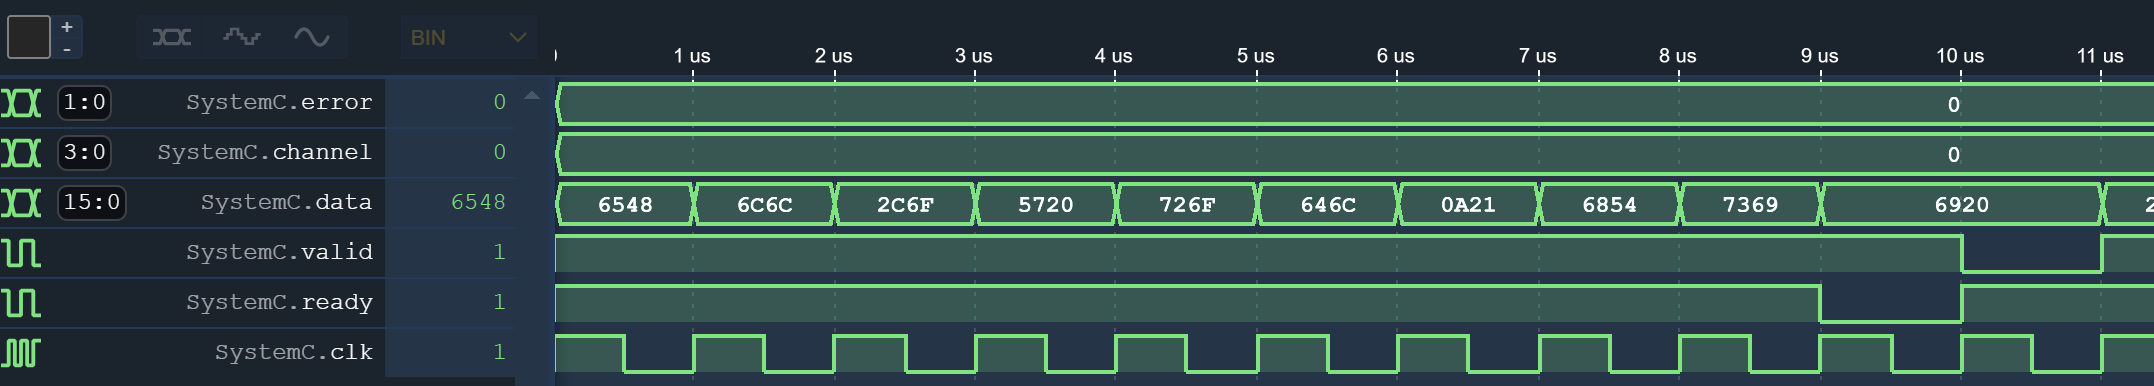
\includegraphics[width=0.95\textwidth]{trace_3_4.png}
    \vspace*{2pt}
    \caption{Trace file, \texttt{DATA\_BITS} = 16.}
\end{figure}

The width of the data channel is adjustable in AvalonConf.hpp. The trace of the same message being sent when \texttt{DATA\_BITS = 64} is shown below.

\begin{figure}[h]
    \centering
    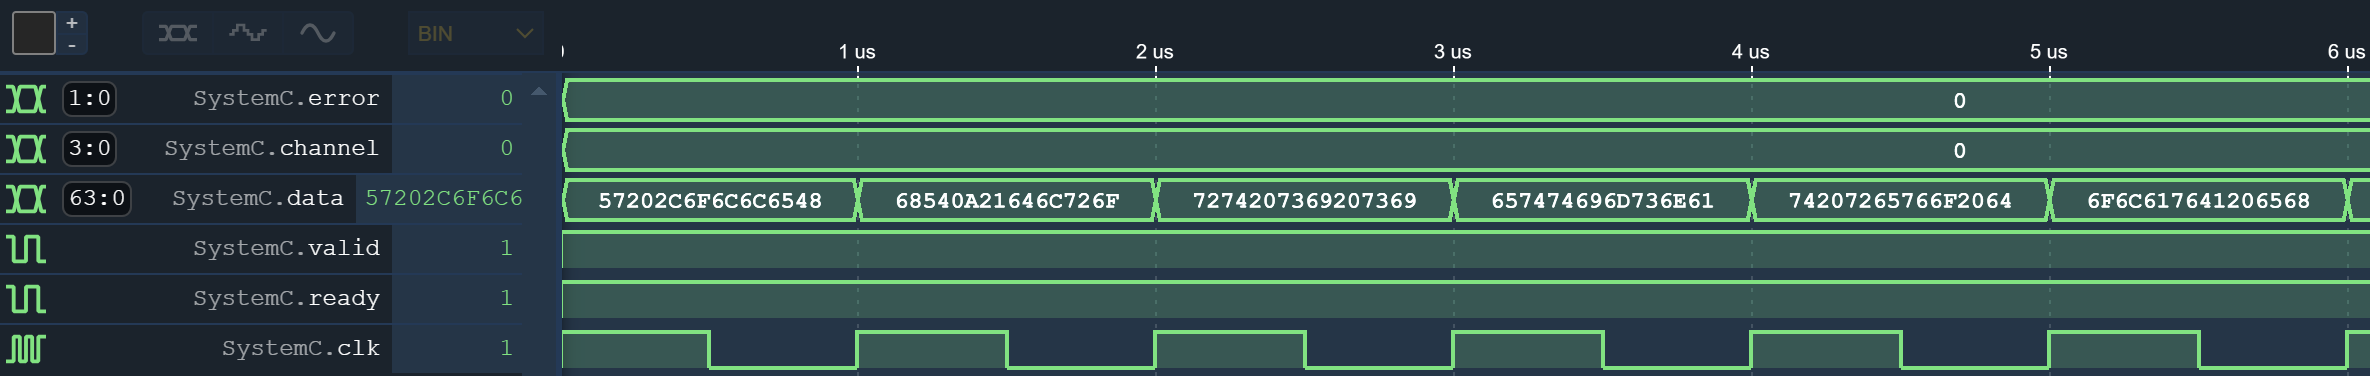
\includegraphics[width=0.95\textwidth]{trace3464.png}
    \vspace*{2pt}
    \caption{Trace file, \texttt{DATA\_BITS} = 64.}
\end{figure}

\newpage

The terminal output is shown below.

\begin{mintedterminal}{a1\_35.exe (DATA\_BITS = 64)}
Transmitting...
RECEIVING
Transmitting...
RECEIVING
Transmitting...
RECEIVING
Transmitting...
RECEIVING
Transmitting...
RECEIVING
Transmitting...
RECEIVING
Transmitting...
RECEIVING
Transmitting...
RECEIVING
RECEIVING
Hello, World!
This is transmitted over the Avalon Streaming Interface!
\end{mintedterminal}


\end{document}